% !TeX program = lualatex
% !TeX encoding = UTF-8
% グローバルチャレンジ2027 II 構築評価報告
% 必須: LuaLaTeX + LuaTeX-ja (TeX Live) / VS Code LaTeX Workshop
\documentclass[a4paper,10pt]{ltjsarticle}
\usepackage[top=19mm,bottom=20mm,left=18mm,right=18mm]{geometry}
\usepackage{graphicx}
\usepackage{hyperref}
\usepackage{url}
\usepackage{titlesec}
\usepackage{indentfirst} % 節・小節直後の段落も字下げする
\hypersetup{hidelinks,pdftitle={グローバルチャレンジ2027 IIにおける構築評価と敗因分析}}
\setlength{\columnsep}{8mm}
\setlength{\parindent}{\zw} % 段落冒頭は全角1文字分の字下げ
\setlength{\parskip}{0pt}
\renewcommand{\baselinestretch}{1.10}
\setlength{\textfloatsep}{9pt plus 2pt minus 2pt}
\setlength{\intextsep}{8pt plus 2pt minus 2pt}
\titleformat{\section}{\normalsize\bfseries}{\thesection.}{0.6em}{}
\titleformat{\subsection}{\normalsize\bfseries}{\thesubsection}{0.6em}{}
\titlespacing*{\section}{0pt}{1.5ex plus .4ex}{.6ex}
\titlespacing*{\subsection}{0pt}{1.1ex plus .3ex}{.4ex}
\pagestyle{plain}

% 編集箇所: 著者名や所属
\newcommand{\PaperAuthor}{ズズくん\qquad gurt}
\providecommand{\PaperAffiliation}{}

\begin{document}
\makeatletter
\twocolumn[
\begin{@twocolumnfalse}
  \begin{center}
    {\Large\bfseries 『Pokémon Champions』グローバルチャレンジ2027 IIにおける\\[1mm]
     構築評価と敗因分析\par}
    \vspace{1.6mm}
    {\normalsize ― トリックルーム軸の環境適合性と戦術の汎用性に関する考察 ―\par}
    \vspace{3mm}
    {\normalsize\PaperAuthor\par}
    {\small\PaperAffiliation\par}
  \end{center}
  \vspace{2mm}
  \noindent\textbf{要旨（Abstract）}\par
  \small
  \noindent 本稿では、『Pokémon Champions』の公式オンライン大会「グローバルチャレンジ2027 II」における使用構築の性能を評価し、成績不振の要因と今後の改善方針について考察する。本大会では、幅広い対戦相手への対応を目的として、メガフラエッテを中心とするスタンダード構築に、リキキリンとコータスによるトリックルーム展開を組み込んだ。しかし、18戦を実施した結果、対戦終了時のレートは初期値と同じ1500にとどまり、前回大会の約1660を大きく下回った。対戦内容を分析した結果、トリックルームの展開困難とコータスの制圧力不足に加え、範囲攻撃の不足、味方との相性補完の不十分さ、相手の行動選択への依存度の高さが問題として認められた。これらの結果から、今後は素早さによる行動順の主導権確保と、相手の行動に依存しにくい範囲攻撃の充実が重要であると結論付けた。\par
  \vspace{1.5mm}
  \noindent\textbf{キーワード：}Pokémon Champions、ダブルバトル、レギュレーションM-C、トリックルーム、リキキリン・コータス、範囲攻撃\par
  \vspace{3mm}\hrule\vspace{3mm}
\end{@twocolumnfalse}
]
\makeatother
\normalsize

\suppressfloats[t] % 最初の左段には上部の図を置かず、右段へ送る。
\section{はじめに}
\subsection{背景}

本大会「グローバルチャレンジ2027 II」は、ポケモンジャパンチャンピオンシップス2027 マスターカテゴリ（以下、PJCS2027）の出場権獲得に向けた公式オンライン大会である。本大会は全6回のグローバルチャレンジ\cite{pjcs}の第2回に該当し、レギュレーションM-Cのダブルバトルによって実施された。上位入賞者にはPJCS2027予選への出場権が付与されるため、対戦成績を安定して積み重ねることが重要となる\cite{pjcs,global2}。

% 図を左段の早い位置で宣言し、右段上部への配置を促す。
\begin{figure}[t]
  \centering
  \IfFileExists{figures/party.png}{%
    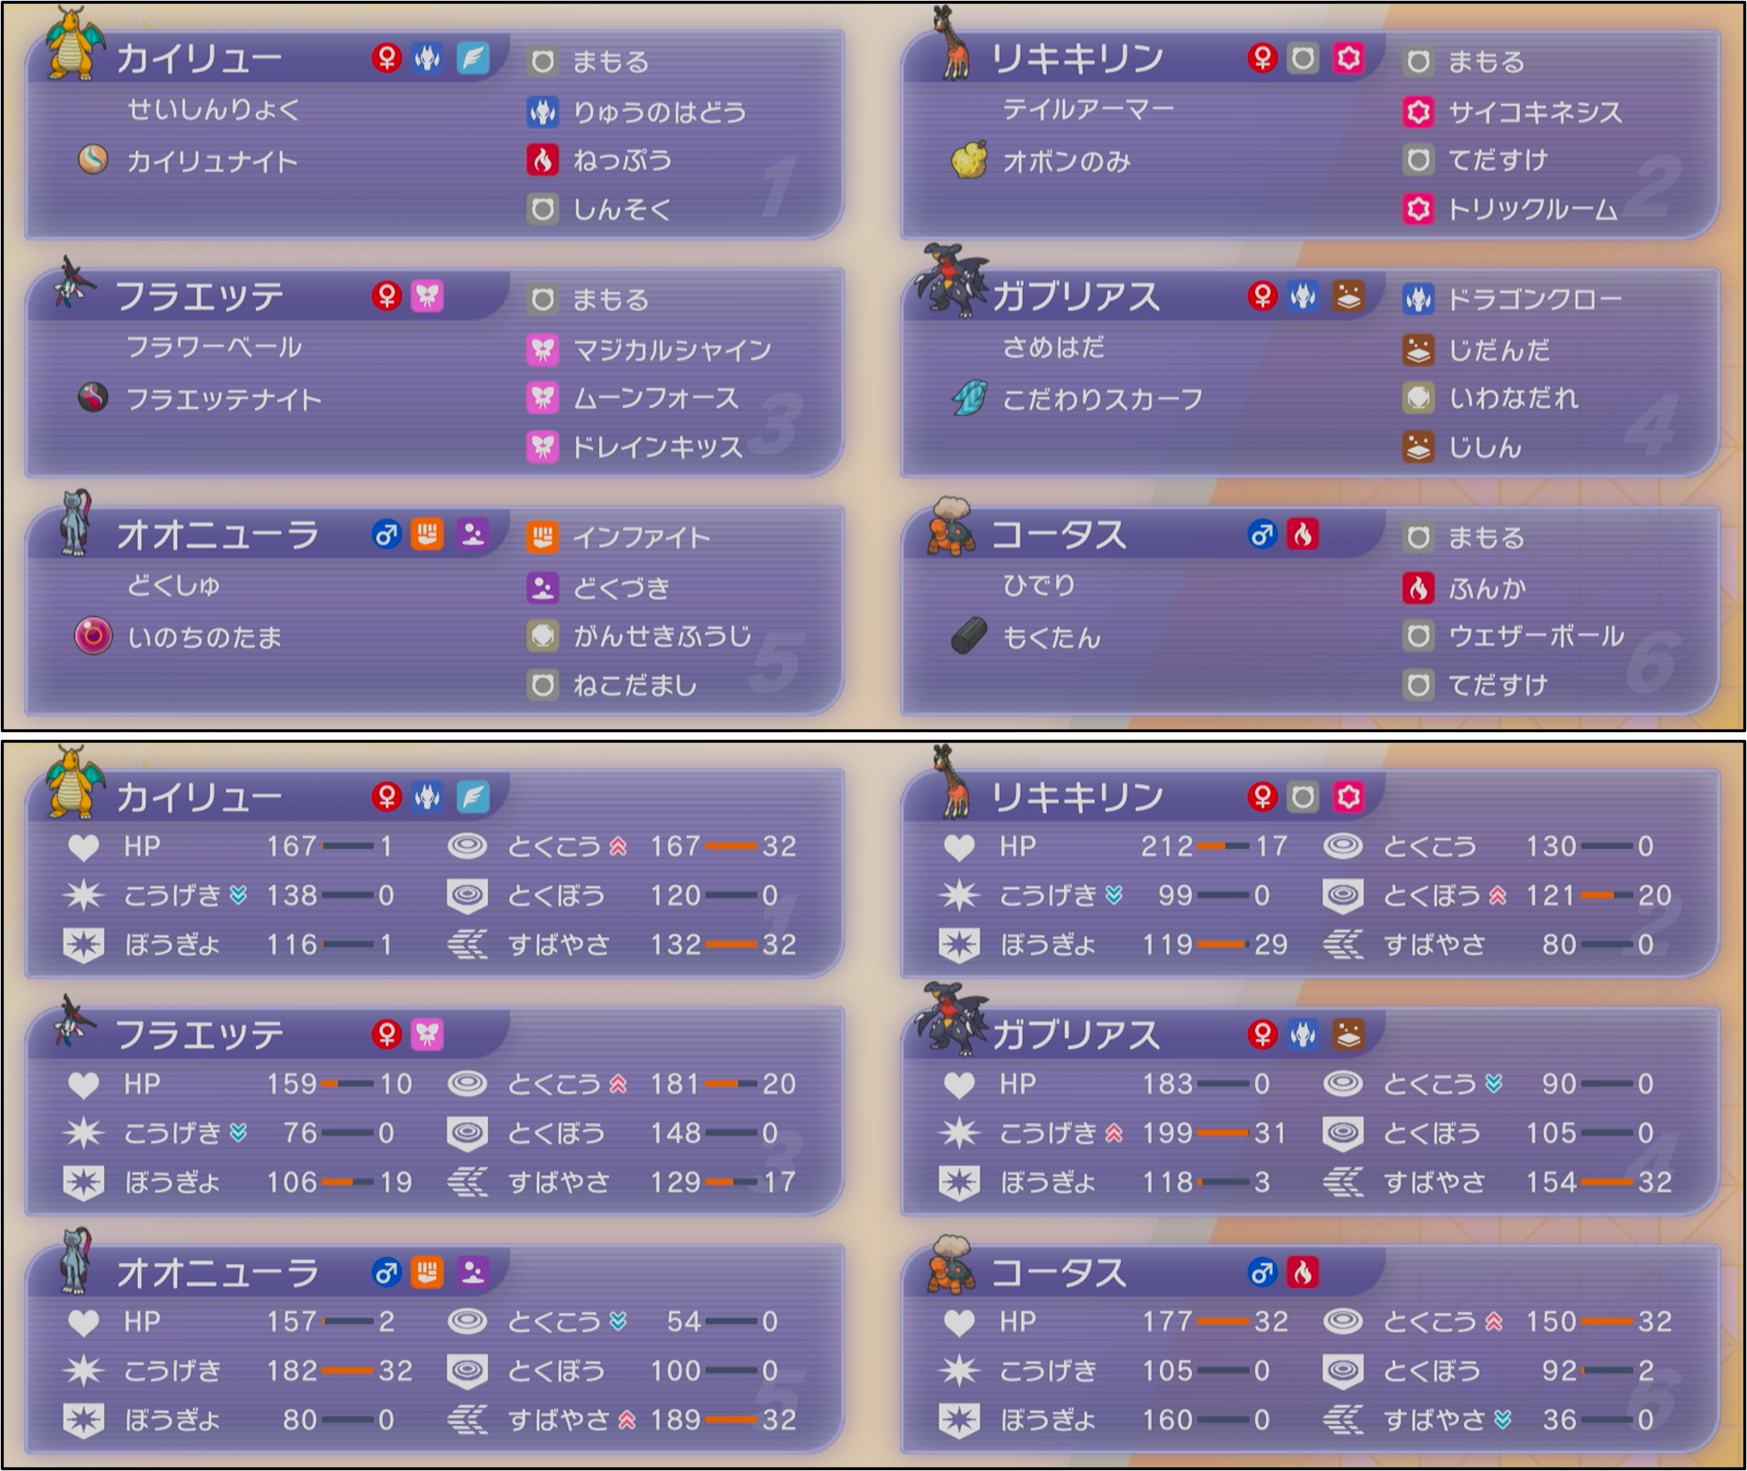
\includegraphics[width=\linewidth]{figures/party.png}%
  }{%
    \fbox{\begin{minipage}[c][37mm][c]{0.92\linewidth}
      \centering\small [ここにパーティ構成の画像]\\[2mm]
      \footnotesize \texttt{figures/party.png} に画像を置くと自動挿入
    \end{minipage}}%
  }
  \caption{グローバルチャレンジ2027 IIで使用した構築}
  \label{fig:party}
\end{figure}

本大会で上位の成績を獲得するためには、幅広い構築に対して高い勝率を維持できるパーティが必要であると考えた。予選突破に必要なレートは1700台半ば程度と予想しており、その水準に到達するには、特定の相手に対する勝率だけでなく、多様な相手に対する安定性が要求される。そのため、構築選択では汎用性と安定性を重視した。

前回の「グローバルチャレンジ2027 I」では、メガボーマンダを中心とした構築を使用し、約1660のレートを記録した。しかし、この成績も想定していた予選突破ラインには届いておらず、さらなる改善が必要であった。そこで今回は、以前のレギュレーションM-Bで使用経験のある構築を基礎とし、操作への習熟度を活かしながら、より安定した立ち回りの実現を目指した。

\subsection{目的}

本稿の目的は、グローバルチャレンジ2027 IIで使用した構築の問題点を明らかにし、今後の大会に向けた改善方針を検討することである。本大会では幅広い相手への対応を意図して構築を変更したものの、レート1500にとどまり、前回大会を大きく下回る成績となった。この結果は、採用した構築が期待した性能を発揮できなかった可能性を示す。

本稿では、成績不振の要因を各ポケモンの役割遂行能力、構築全体の相性補完、および戦術の安定性の観点から分析する。また、前回大会で使用したメガボーマンダ軸との比較を通じて、構築設計上の問題点を整理する。これにより、今回の敗因を検討するとともに、今後の改善に向けた指針を導出する。

\section{使用構築と評価方法}
\subsection{構築方針}

本大会では、幅広い相手に柔軟に対応できるスタンダード構築を基本方針として採用した。スタンダード構築は特定の展開の成立だけに依存せず、盤面に応じて攻撃や交代を選択し、継続的に有利な状況を形成することを目指す。本大会のように高い勝率が要求される条件では、相手の構築によって勝ち筋が極端に制限されることを避ける必要があるため、この方針が適切であると判断した。

構築の中心にはメガフラエッテを採用し、補助的な勝ち筋としてリキキリンとコータスによるトリックルーム展開を組み込んだ。コータスは特性「ひでり」による晴れ状態と、HP残量が多いほど威力が高くなる「ふんか」を組み合わせることで、相手全体に大きなダメージを与えられる。また、リキキリンの「てだすけ」でコータスの攻撃性能をさらに高められる。この組み合わせを制圧手段としつつ、残りのポケモンによって攻撃範囲と対応可能な相手を補完した。

今回の構築は、以前のレギュレーションM-Bで使用していた構築を基礎としている。筆者は当時の構築に一定の習熟度を有しており、各ポケモンの役割と基本的な立ち回りを把握していた。そのため、新たな構築を一から習得する場合と比較して、対戦中の判断負担を抑えられることも採用理由の一つであった。

\subsection{使用パーティ}



本構築は、メガフラエッテ、メガカイリュー、リキキリン、ガブリアス、オオニューラ、コータスの6匹で構成される（図\ref{fig:party}）。メガフラエッテとメガカイリューを相手に応じて選択するメガシンカ候補として採用し、リキキリンとコータスのトリックルーム展開を補助的な勝ち筋とした。また、ガブリアスの攻撃性能と技範囲、オオニューラの「ねこだまし」による行動制限を組み合わせ、トリックルームに依存しない立ち回りも可能になることを想定した。

\subsection{評価方法}

本稿では、レートの変動と対戦中の使用感に基づき、各ポケモンの役割遂行能力および構築全体の有効性を定性的に評価する。具体的には、想定した役割を遂行できたか、構築内の相性補完によって個々の性能を引き出せたか、相手の行動選択に依存せず安定した勝ち筋を形成できたかという観点から分析する。また、以前のレギュレーションM-Bで有効だった戦術が、M-Cでも機能するかを検討する。

本稿では、大会環境全体の分析ではなく、今回の対戦経験に基づく構築評価に対象を限定する。対戦ごとの勝敗数や選出率の詳細な記録は取得していないため、統計的な比較ではなく、対戦中に観測された事象を中心とする。また、対戦相手は主にレート1500付近に限られることから、大会環境全体の構築分布は分析しない。

\section{結果}
\subsection{大会成績}

本大会では計18戦を実施し、対戦終了時のレートは初期値と同じ1500であった。勝敗数の詳細は記録していないが、レートが初期値からほとんど変動していないことから、勝率は概ね50\%前後であったと推測される。ただし、レートの変動量は相手のレートにも依存するため、正確な勝率は不明である。

今回の最終レートは、前回大会の約1660と比較して約160低い結果となった。また、予選突破に必要と予想していた1700台半ばにも大きく届かなかった。この結果から、今回の構築では上位の成績を目指すうえで必要な勝率を確保できなかったことが確認された。

\subsection{トリックルーム軸の運用結果}

リキキリンとコータスを中心としたトリックルーム展開は、期待した性能を十分に発揮できなかった。リキキリンは特性「テイルアーマー」で先制技を防ぎつつ、「トリックルーム」や「てだすけ」で味方を支援する役割を想定していた。しかし実際には、相手の高火力攻撃によって「トリックルーム」を使用する前に倒される場面や、「ふういん」によって技の使用を封じられる場面が見られた。

トリックルームが成立した場合であっても、コータスによる制圧は十分に機能しなかった。特に、雨状態への天候変更に加え、レギュレーションM-B当時よりもほのおタイプの攻撃に耐性を持つ相手が増加していたという対戦上の印象から、「ふんか」で相手を倒しきれない場面が見られた。その結果、コータスは高火力の範囲攻撃役として機能せず、実質的に天候を晴れへ変更する役割にとどまることが多かった。

コータスの制圧力不足に伴い、リキキリンも十分な役割を遂行できなかった。リキキリンは自身の攻撃性能が低いため、味方への支援によって盤面に貢献する必要がある。しかし、コータスの「ふんか」が有効に機能しない場合、「てだすけ」による火力補助も十分な効果を発揮できず、相手への圧力が乏しい状態となった。

\subsection{メガフラエッテの運用結果}

メガフラエッテは、構築内で比較的安定した性能を示した。対面する相手に対して有効な行動を選びやすく、特定の相手に極端に不利となる場面も比較的少なかった。そのため、相手の構築に応じた選出の自由度が高く、スタンダード構築の中心として想定した役割を果たした。

「ドレインキッス」の採用によって、メガフラエッテの継戦能力が向上した。従来の「はめつのひかり」を「ドレインキッス」に変更したことで、攻撃と回復を両立でき、継続的に相手へ圧力をかける性能が改善した。一方、「はめつのひかり」の高い瞬間火力を失ったことで、通常の攻撃では突破困難な相手への強引な突破手段は減少した。

\subsection{メガカイリューの運用結果}

メガカイリューは、特性「マルチスケイル」による耐久性能を活かし、安定した盤面形成に寄与した。「マルチスケイル」はHP満タン時に受けるダメージを半減するため、弱点を突かれる攻撃に対しても耐えられる場面が多く、特に初手の盤面形成に適していた。一方、相手を短時間で倒しきる火力には不足を感じる場面があり、継続的に攻撃できる盤面を整える必要があった。

メガカイリューの主要な攻撃手段の一つである「ねっぷう」は範囲攻撃として有効であった一方、命中不安による損失が問題となった。「ねっぷう」は相手2体に同時にダメージを与えられるため、実際の対戦でも使用する機会が多かった。しかし、命中率が90\%であり、一定の確率で攻撃が失敗する。特に、はがねタイプやこおりタイプのポケモンに対して使用する場合、外したことで相手の反撃を許し、そのままメガカイリューが倒される場面が見られた。

\subsection{ガブリアスの運用結果}

ガブリアスは単体性能の高さを示した一方、構築全体との相性補完に課題が認められた。ドラゴン・じめんタイプによる耐性に加え、「じだんだ」「ドラゴンクロー」「いわなだれ」「じしん」による広い攻撃範囲は優秀であり、さまざまな相手に有効な攻撃手段を確保できた。特に「いわなだれ」が有効な相手の並びでは、2体同時への削りに加えて追加効果による「ひるみ」が強力に機能した。

一方、「じしん」は味方との相性上の制約によって十分に活用できなかった。今回の構築では、味方にじめんタイプの攻撃を無効化できるポケモンがカイリューしか存在せず、「じしん」を選択できる場面が大きく制限された。そのため、強力な範囲攻撃としての性能を十分に発揮できなかった。

\subsection{オオニューラの運用結果}

オオニューラは「いのちのたま」による火力強化を採用したものの、期待した攻撃性能を十分に発揮できなかった。以前と比較して特性「いかく」を持つポケモンに遭遇する機会が増え、攻撃を下げられた状態では「いのちのたま」を持っていても相手を倒しきれず、反撃によって倒される場面が見られた。また、サイコフィールドと「ワイドフォース」を組み合わせた構築に対しては、エスパータイプの攻撃で弱点を突かれやすく、行動回数を確保することが困難であった。

一方、オオニューラには場に残って継続的に攻撃する運用に改善の余地が認められた。実際の対戦では、瞬間火力を高めても相手を倒しきれない場面が多く、その後の反撃で倒されることが問題となった。そのため、攻撃性能を維持しながら行動回数を増やせれば、より効果的に運用できる可能性が示された。

\subsection{構築全体の攻撃性能}

本構築では、高火力の範囲攻撃を安定して使用することが困難であった。本来はコータスの「ふんか」を主要な範囲攻撃として想定していたが、前述の理由によって使用機会と有効性が制限された。また、ガブリアスの「じしん」も味方との相性上の制約が大きく、安定して使用できる範囲攻撃はメガフラエッテの「マジカルシャイン」に偏っていた。

範囲攻撃による制圧力の不足は、相手の行動を予測する必要がある場面の増加につながった。「マジカルシャイン」は安定した範囲攻撃だが、晴れ状態の「ふんか」と比較すると瞬間的な制圧力は低い。そのため、相手2体のうち一方を倒さなければ不利になる盤面では、どちらを攻撃するかという択が頻繁に発生し、選択を誤るとそのまま敗北につながる場面が見られた。

\section{考察}
\subsection{トリックルーム軸の環境適合性}

今回の成績不振の主要な要因の一つは、リキキリンとコータスを中心としたトリックルーム軸の環境適合性が低下していたことである。レギュレーションM-Bでは、リキキリンによってトリックルームを成立させ、コータスの晴れ状態の「ふんか」を「てだすけ」で強化する戦術が有効に機能していた。しかし今回の対戦では、相手の高火力攻撃や「ふういん」による展開阻害によって、トリックルームの成立自体が困難となる場面が増加した。これは、少なくとも筆者が対戦した範囲では、高火力のポケモンや展開阻害手段がトリックルーム軸に与える影響が大きくなったことを示唆する。

トリックルーム軸の有効性が低下したもう一つの要因は、展開後のコータスの制圧力不足である。今回の対戦では、雨を利用する構築に加え、レギュレーションM-B当時と比較して、ほのおタイプの攻撃に耐性を持つ相手が増加していた。このため「ふんか」によって相手を一掃することが難しく、トリックルームを成立させるために要した行動に見合う成果を得られない場面が多かった。

コータスの攻撃性能がトリックルームに強く依存していたことも、構築の安定性を損なう要因となった。「ふんか」はHP残量が多いほど威力が高いため、コータスが後攻する場合、攻撃前の被弾によって威力が低下する危険性が高い。極めて素早さの低いコータスは、トリックルームが成立しなければ基本的に後攻となり、その攻撃性能を発揮しにくい。したがって、展開に失敗すると大きく不利になる一方、成功しても十分な制圧力が保証されないという構造的な問題が存在した。

リキキリンとコータスの相互依存関係は、トリックルーム軸の不安定さをさらに増大させていた。リキキリンは「トリックルーム」や「てだすけ」でコータスを支援するが、コータスの攻撃が有効に機能しない場合、リキキリン自身の低い攻撃性能が顕在化し、相手へ圧力をかけられなくなる。両者の組み合わせは、一方の役割が機能しなかった場合に、もう一方の役割も同時に失われやすい構造となっていた。

以上より、今回のトリックルーム軸は展開の成立条件が厳しい一方、成立後に得られる利益も小さくなっていたと考えられる。この問題は個々のポケモンの性能不足だけでは説明できず、リキキリンとコータスを組み合わせる構築方針そのものに起因する。少なくとも今回遭遇した相手に対しては、両者を中心とした構築は適切ではなかった可能性が高い。

\subsection{素早さ操作と行動順の主導権}

ダブルバトルでは、相手より先に行動することで、攻撃だけでなく盤面全体の主導権を確保できる。相手の攻撃を受ける前にポケモンを倒したり、追加効果で相手の行動を阻害したりすることで、相手の予定した行動を成立させずに有利な状況を形成できるためである。このことから、行動順の主導権は盤面を安定して有利に維持するための重要な要素となる。

今回採用した「トリックルーム」は、展開時に相手へ行動の主導権を渡しやすい点で問題があった。成立後に素早さの低いポケモンから行動できる強力な技であるが、技の優先度が低いため、展開するターンには相手からの攻撃や妨害を受けやすい。特に相手の高火力攻撃や「いわなだれ」による「ひるみ」が脅威となり、成立前に行動を阻害される危険性が高かった。展開を阻害された場合、コータスを中心とした構築ではその後の主導権を取り戻すことも困難であった。

行動順の主導権を確保するためには、「おいかぜ」のような能動的な素早さ操作が有効であると考えられる。「おいかぜ」は味方の素早さを高め、相手より先に攻撃できる状況を形成しやすくする。これにより、相手の攻撃を受ける前にポケモンを倒すだけでなく、「いわなだれ」などの追加効果によって相手の行動を阻害する機会も増加する。

今回の構築では「トリックルーム」への依存度を低減し、先制して攻撃できる手段を増やすことが有効であると考えられる。「おいかぜ」も展開を妨害され得るため常に優れているわけではないが、今回の構築ではトリックルーム成立後も十分な制圧力を発揮できなかった。したがって、より能動的な素早さ操作への変更が望ましい。

\subsection{範囲攻撃の不足と戦術の安定性}

今回の構築では、高火力の範囲攻撃の不足によって相手の行動選択への依存度が高くなっていたと考えられる。ダブルバトルでは、相手2体がそれぞれ異なる行動を選択できるため、単体攻撃で一方を倒す必要がある場合、どちらの行動が脅威となるかを予測しなければならない。しかし、相手の攻撃対象や「まもる」、交代によって最適な行動が変わる場合があり、予測を誤ると大きな損失が生じる。

高火力の範囲攻撃は、相手の行動選択への依存度を低減する手段として有効である。相手のどちらが行動するかにかかわらず、両方にダメージを与えられるため、予測が外れた場合でも一定の成果を確保しやすい。特に相手2体を同時に倒せる可能性のある盤面では、相手の行動候補を広くカバーできる。

前回大会のメガボーマンダ軸では、高火力の範囲攻撃と素早さによって相手の行動選択への依存度を抑えられていた。具体的には、サーフゴーの「ゴールドラッシュ」が強力な範囲攻撃として機能し、構築全体にも素早さと攻撃性能の高いポケモンが多かった。そのため、相手より先に攻撃し、択を発生させる前に盤面を有利にできる場面が多かった。一方、今回はコータスの「ふんか」が機能せず、範囲攻撃の制圧力が大幅に低下した。

以上より、範囲攻撃の価値は総ダメージ量だけでなく、行動予測を誤った場合にも一定の成果を得られる戦術上の安定性にあると考えられる。今回の構築ではこの性質を持つ攻撃手段が不足し、幅広い相手への安定した対応が難しくなっていた。今後は範囲攻撃の安定した使用を、構築の汎用性を評価する重要な要素として位置付ける必要がある。

\subsection{高レート帯への過学習と戦術の汎用性}

今回の構築および立ち回りは、ランクマッチにおける一定以上のレート帯の相手に過度に適応していた可能性がある。高レート帯では相手の合理的な行動選択や一定の対戦傾向を仮定し、リスクとリターンを評価した行動選択が成立しやすい。しかし、今回対戦したレート1500付近では想定と異なる行動を取られることがあり、予測を前提とした立ち回りが安定しなかった。

特定の対戦傾向への過度な適応は、機械学習における過学習（overfitting）に類似した現象として解釈できる。機械学習では特定のデータに過度に最適化すると、未知のデータへの予測性能が低下する場合がある。今回の対戦でも、高レート帯で成立していた行動予測が、異なる行動傾向の相手には機能しなかった可能性がある。ただし、レート帯ごとの勝率を定量比較していないため、この説明は対戦経験に基づく仮説にとどまる。

相手の行動傾向に依存しない戦術の確保が、構築の汎用性を高めるために重要である。相手が複数の行動候補から何を選んでも一定の利益が得られる範囲攻撃や、相手より先に行動して主導権を確保する手段が必要となる。前節で述べた範囲攻撃と素早さの確保は、このような予測への依存度を低減するために有効である。

以上より、構築の強さは特定の相手への最大性能だけでなく、異なる行動傾向の相手に対しても勝ち筋を維持できるかという観点から評価する必要がある。今回の構築は想定外の行動に対する頑健性が不足していた可能性がある。

\subsection{メガフラエッテとメガカイリューの性能評価}

メガフラエッテは、スタンダード構築の中心に求められる汎用性と継戦能力を備えていると考えられる。相手に応じて攻撃対象や技を選択し、有利な状況を形成しやすいため、選出が大きく制限される場面も少なかった。「ドレインキッス」の採用で継戦能力が向上した一方、「はめつのひかり」の瞬間火力も突破困難な相手への重要な手段であるため、今後も両者の比較が必要である。

メガカイリューは、耐久性能を活かした安定性に優れる一方、瞬間的な攻撃性能に課題があると考えられる。「マルチスケイル」による耐久性能は初手の盤面形成に有効だったが、相手を短時間で倒しきる火力には不足を感じる場面があった。このため、メガフラエッテと比較して、継続的に攻撃できる盤面を整えることへの依存度が高い。

メガカイリューの「ねっぷう」は優秀な範囲攻撃であるものの、命中不安と攻撃失敗時の損失を考慮する必要がある。「ねっぷう」は相手2体へ同時にダメージを与えられ、メガカイリューでも使用する機会が多かった。しかし、メガカイリューはほのおタイプではないため、タイプ一致による威力補正を受けられない。また、命中しなかった場合には相手の反撃を許すことになり、攻撃失敗によって不利になる状況を考慮した技選択が必要となる。

「ねっぷう」を高火力で使用できる代表的なポケモンとして、メガリザードンYが挙げられる。メガリザードンYは特性「ひでり」でほのおタイプの攻撃を強化できることに加え、タイプ一致による威力補正と、メガカイリューより高い特攻を持つことから、「ねっぷう」でより大きなダメージを与えられる。したがって、同じ技でも相手に与える圧力には大きな差が存在する。

メガカイリューは、メガリザードンYと比較して「ねっぷう」が命中しなかった場合の損失が大きくなりやすい。メガカイリューは、攻撃対象となることの多いはがねタイプやこおりタイプのポケモンに対して防御面で不利になりやすく、攻撃を外した場合にそのまま倒される危険性が高い。一方、メガリザードンYはほのお・ひこうタイプによってこれらの相手に比較的有利な耐性を持ち、一度の攻撃失敗を許容できる場面がある。

以上より、命中不安のある攻撃技の評価では、威力や攻撃範囲に加え、攻撃失敗時の損失も考慮する必要がある。範囲攻撃を主要な勝ち筋とする場合、その技を使用するポケモンが反撃をどの程度許容できるかが重要である。

\subsection{ガブリアスの相性補完とオオニューラの継戦能力}

ガブリアスの運用上の問題は、単体性能ではなく構築内の相性補完が不十分だったことに起因すると考えられる。「じしん」は強力な範囲攻撃だが味方にも攻撃が及ぶため、じめんタイプの攻撃を無効化できる味方との組み合わせが重要となる。今回の構築ではカイリュー以外にその役割を担えるポケモンが存在せず、「じしん」を積極的に選択できる盤面が限られていた。

オオニューラについては、瞬間火力よりも場に残って攻撃できる回数を増やす方が有効だった可能性がある。「いかく」で攻撃を下げられた場合、「いのちのたま」による強化だけでは相手を倒しきれず、反撃や反動ダメージで行動回数が減少する。このため、単発のダメージ量よりも継続して攻撃できる機会の確保が重要であったと考えられる。

これらの結果は、個々のポケモンの性能だけでなく、その性能を引き出す構築全体の設計が重要であることを示している。ガブリアスでは攻撃技を使用できる盤面の確保が、オオニューラでは攻撃機会の確保が課題となった。今後は単体性能に加え、味方との相性補完と実際の行動回数を含めた評価が必要である。

\section{今後の構築改善方針}
\subsection{トリックルームへの依存度の低減}

今後の構築改善で最も優先すべき課題は、リキキリンとコータスを中心としたトリックルーム軸の再検討である。今回の対戦では、展開の成立条件が厳しく、成立後の制圧力も不足していた。特にコータスが高火力の攻撃役として機能せず、天候変更を主な役割としていたことは、構築内の役割配分に改善の余地があることを示す。

今後は、トリックルームの成立を前提とせず、相手より先に攻撃して有利な盤面を形成する構築への変更を検討する。これにより特定の展開が成立しない場合でも攻撃性能を維持しやすくなり、相手の妨害手段への頑健性の向上が期待できる。

\subsection{「おいかぜ」による素早さ操作の導入}

素早さ操作の代替手段として「おいかぜ」の導入を検討する。「おいかぜ」で先に行動できる状況を形成すれば、相手から攻撃を受ける前にポケモンを倒せる機会が増える。また「いわなだれ」などの追加効果を持つ攻撃を先に使用すれば、相手の行動を阻害する展開も期待できる。

「おいかぜ」による素早さの優位性は、攻撃性能だけでなく盤面の主導権維持にも寄与すると考えられる。先に行動することで、相手からの攻撃や妨害を受ける前に有利な状況を形成できるためである。今後は、先制のための手段と高火力の攻撃手段を組み合わせることを重視する。

\subsection{高火力の範囲攻撃の確保}

今後の構築では、高火力の範囲攻撃を安定して使用できることを重視する。今回の構築ではコータスの「ふんか」が機能せず、相手2体のうち一方を倒す盤面で攻撃対象の予測を強いられた。この問題を改善するためには、相手の行動に依存せず両方のポケモンへ圧力をかけられる技が必要である。

範囲攻撃の性能を引き出すためには、技そのものの強さだけでなく味方との相性補完も重要となる。今回のガブリアスの「じしん」のように、味方への被害によって使用が制限される場合、強力な技でも実質的な攻撃手段として機能しない。そのため、範囲攻撃を安定して使用できる盤面を構築全体で形成できるかを評価する。

\subsection{「いわなだれ」に対する対策の強化}

「いわなだれ」への対策では、被ダメージの軽減だけでなく、相手の技選択にリスクを与えることが重要である。「いわなだれ」は範囲攻撃の削り性能に加え、命中した相手を30\%の確率でひるませる追加効果を持つ。このため、単にダメージを耐えるだけでは十分な対策とならず、先制されてひるむ危険性が残る限り、有利な盤面から逆転され得る。

「いわなだれ」の使用を抑制する手段として、「ワイドガード」による防御や、ブリジュラスのようにいわタイプの攻撃を受けながら戦えるポケモンの採用が考えられる。ただし、ブリジュラスの耐性や特性「じきゅうりょく」は「ひるみ」自体を防ぐわけではなく、被ダメージ軽減と行動保証は別に評価する必要がある。

今後は、相手が安易に「いわなだれ」を選ぶと不利益が生じる構築を目指す。単に攻撃を耐えるだけでなく相手の技選択に制約を与えられれば、行動を一定程度制御でき、盤面の安定性を高められると考えられる。

\subsection{メガリザードンYによる役割の統合}

メガリザードンYの採用は、メガカイリューとコータスの役割を統合し、構築枠を確保するための改善案である。メガリザードンYは特性「ひでり」による天候変更と、高い特攻からのほのおタイプの範囲攻撃を両立できる。このため、天候変更役のコータスと範囲攻撃役のメガカイリューの役割を1匹に集約できる可能性がある。

メガリザードンYは、メガシンカによる天候変更のタイミングを利用して雨構築への対抗手段を確保できる。メガシンカ時に「ひでり」が発動するため、通常の交代による天候変更とは異なるタイミングで晴れを形成できる。交代による特性の発動がメガシンカより先に処理される状況では、相手が交代によって雨を形成した場合も、その後のメガシンカで晴れに変更できる。

一方、メガリザードンYの採用にはメガフラエッテとのメガシンカ枠の競合が存在する。メガシンカは1回の対戦につき1匹しか使用できないため、メガリザードンYを使用した場合、同じ対戦でメガフラエッテを使用できない。今回の構築では晴れ状態のメガフラエッテも有効な勝ち筋であり、雨構築に対して天候を変更してからメガフラエッテを通す戦術を失う可能性がある。

メガリザードンYの採用は、構築全体の役割配分と勝ち筋の再設計として検討する必要がある。メガフラエッテ中心の戦術を維持するか、メガリザードンYの高火力の範囲攻撃を新たな中心とするかによって残りの役割も変化するため、単純なポケモンの入れ替えではなく、構築全体の検証が必要である。

\subsection{オオニューラの持ち物と運用方針}

オオニューラは「いのちのたま」による瞬間火力重視から、行動回数を増やす持ち物への変更を検討する。今回の対戦では「いかく」や反撃によって十分な攻撃回数を確保できなかった。単発の火力よりも継続して攻撃できる能力を確保する方が、結果として与える総ダメージ量を増やせる可能性がある。

持ち物の候補として「きあいのタスキ」や各種シードが挙げられる。「きあいのタスキ」はHP満タン時の一撃によるひんしを防ぎ、追加の行動機会を確保できる可能性がある。一方、シードを使うには対応するフィールドの確保が前提となるため、構築全体との整合性を検証する必要がある。今後は単発の攻撃性能だけでなく、確保できる行動回数を含めて持ち物を評価する。

\subsection{メガフラエッテの技構成}

メガフラエッテは「ドレインキッス」による継戦能力と「はめつのひかり」による突破性能の比較を継続する。「ドレインキッス」は攻撃と回復を両立でき、盤面に残りながら相手に圧力をかける運用に適する。一方、「はめつのひかり」は高い瞬間火力によって相手を強引に突破でき、通常の攻撃では突破困難な相手への対抗手段として有効である。

両者の優劣は、構築全体でメガフラエッテに求める役割によって変化すると考えられる。継戦能力を重視する構築では「ドレインキッス」が有効な一方、瞬間的な突破性能を必要とする場合は「はめつのひかり」の価値が高まる。今後は両者を比較し、構築全体の勝ち筋に合う技を選択する。

\section{本分析の限界}

本稿の分析には、対戦数と取得データの制約が存在する。評価対象は18戦であり、勝敗数、選出率、技の使用回数などの詳細な記録は取得していない。このため、各要因が勝率に与えた影響を定量評価できず、示した問題点は主に対戦中の観察に基づく。

今回の対戦結果から、レギュレーションM-C全体の傾向を一般化することはできない。相手は主にレート1500付近に限られ、遭遇したポケモンや戦術が環境全体を代表しているとは限らない。雨構築やほのおタイプの攻撃に耐性を持つポケモンの増加についても、筆者の経験に基づく評価であり、大会全体の使用率による検証を経ていない。

前回大会との成績差についても、構築変更のみを原因と断定することはできない。両大会は同じレギュレーションM-Cであったが、使用構築、対戦相手、対戦数が異なる。レート差には構築性能だけでなく相手との組み合わせや行動選択も影響し得るため、今回の分析は原因の確定ではなく改善に向けた仮説の整理と位置付けられる。

今後の分析では、対戦ごとの詳細な記録を蓄積して改善効果を客観的に評価する必要がある。具体的には、勝敗、選出、トリックルームの成立率、範囲攻撃の使用回数、敗北の直接的な要因を記録する。これらを蓄積すれば改善案の有効性をより定量的に検討できる。

\section{結論}

本大会における成績不振の主要な要因は、トリックルーム軸の環境適合性の低下と、構築全体の攻撃性能および戦術の安定性の不足にあったと考えられる。今回の構築は幅広い相手に対応できるスタンダード構築を目指したが、リキキリンとコータスによる展開への依存度が高く、成立条件と展開後の制圧力の双方に問題が存在した。また高火力の範囲攻撃が不足し、相手の行動を正確に予測しなければ有利な盤面を維持できない場面が増加した。

今回の構築では、個々のポケモンの性能を構築全体として十分に引き出せていなかった可能性が高い。メガフラエッテ、メガカイリュー、ガブリアスにはそれぞれ一定の有効性が認められたが、味方との相性補完や攻撃機会の確保が不十分で、能力を発揮できない場面があった。このことから、各ポケモンの役割が相互に機能する設計が必要であると考えられる。

今後の改善では、素早さによる行動順の主導権確保と、高火力の範囲攻撃の充実を優先する。「おいかぜ」などの素早さ操作、範囲攻撃の安定した使用、「いわなだれ」への対策を中心に構築を改善し、相手の行動を正確に予測する必要がある場面を減らすことを目指す。

以上の考察から、今後の構築設計では特定の相手への最大性能だけでなく、幅広い対戦相手に対して安定して性能を発揮できる汎用性と頑健性の確保が重要であると結論付けた。想定外の行動に対しても一定の成果を得られる戦術を重視することが、今後の大会成績の安定化につながると考えられる。

\begin{thebibliography}{9}
\bibitem{pjcs} 株式会社ポケモン，「『Pokémon Champions』チャンピオンシップシリーズ『2027シーズン』について」，『Pokémon Champions』公式お知らせ．\url{https://champions-news.pokemon-home.com/ja/page/833.html}
\end{thebibliography}
\end{document}
